\documentclass[pdf, unicode, 12pt, a4paper,oneside,fleqn]{article}

\usepackage{styles/log-style}
\begin{document}

\begin{titlepage}
\begin{center}
\bfseries
{\Large Московский авиационный институт\\ (национальный исследовательский университет)}

\vspace{48pt}
{\large Факультет информационных технологий и прикладной математики}

\vspace{36pt}
{\large Кафедра вычислительной математики и программирования}

\vspace{48pt}Лабораторная работа \textnumero 3 по курсу 
\enquote{Численные методы}
\end{center}
\vspace{72pt}

\begin{flushright}
\begin{tabular}{rl}
Студент: & П.\,А. Гамов \\
Преподаватель: & Д.\,Л. Ревизников \\
Группа: & М8О-407Б \\
Дата: & \\
Оценка: & \\
Подпись: & \\
\end{tabular}
\end{flushright}
\vfill
\begin{center}
\bfseries
Москва, \the\year
\end{center}
\end{titlepage}

\pagebreak

\section{Приближение функций}

\begin{lstlisting}
def f(x):
    return 1/tan(x)
    
x_a = [pi/8, 2*pi/8, 3*pi/8, 4*pi/8]
y_a = [f(_) for _ in x_a]

x_b = [pi/8, 5*pi/16, 3*pi/8, pi/2]
y_b = [f(_) for _ in x_b]

x_star = pi/3
y_star = f(x_star)
\end{lstlisting}

\subsection{Newton}

\begin{lstlisting}
def divided_diff(x, y):
    n = len(y)
    coef = []
    for i in range(len(x)):
        r = [y[i]]
        for j in range(len(x)-1):
            r.append(0)
        coef.append(r)
    for j in range(1,n):
        for i in range(n-j):
            coef[i][j] = (coef[i+1][j-1] - coef[i][j-1]) / (x[i+j]-x[i])
    return coef
    
def Newton(X, x, y):
    coef = divided_diff(x, y)
    res, cof = coef[0][0], []
    for i in range(1,len(coef)):
        cof.append(coef[0][i])
    for i in range(len(cof)):
        for j in range(i+1):
            cof[i] *= (X - x[j])
        res += cof[i]
    return res
\end{lstlisting}

\subsection{Lagrange}

\begin{lstlisting}
def Lagrange(X,x,y):
    res = 0
    for i in range(len(x)):
        f_i = y[i]
        for j in range(len(y)):
            if j != i:
                f_i *= (X - x[j]) / (x[i] - x[j])
        res += f_i
    return res
\end{lstlisting}

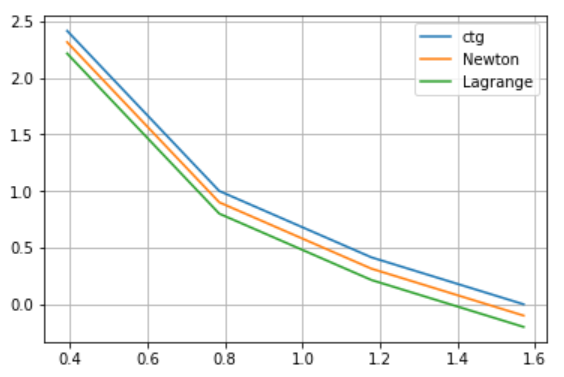
\includegraphics[scale=0.5]{data1.png}

\subsection{Cubic spline}

\begin{lstlisting}
x = [1,1.9,2.8,3.7,4.6]
y = [2.4142,1.0818,0.50953,0.11836,-0.24008]

x_star = 2.66666667
\end{lstlisting}

\begin{lstlisting}
def cubic_spline(x,y,X=None):
    h = [x[i]-x[i-1] for i in range(1, len(x))]
    M = [[h[i-1], 2.0*(h[i-1]+h[i]), h[i]] for i in range(1, len(h))]
    M[0][0] = M[-1][2] = 0.0
    b = [3.0*((y[i+1]-y[i])/h[i]-(y[i]-y[i-1])/h[i-1]) for i in range(1, len(h))]
    P = [-elem[2] for elem in M]
    Q = [elem for elem in b]
    P[0] /= M[0][1]
    Q[0] /= M[0][1]
    for i in range(1, len(b)):
        z = (M[i][1] + M[i][0] * P[i-1])
        P[i] /= z
        Q[i] -= M[i][0] * Q[i-1]
        Q[i] /= z
    x_ = [item for item in Q]
    for i in range(len(x_) - 2, -1, -1):
        x_[i] += P[i] * x_[i + 1]
    c = [0.0] + x_
    a = list(y[:len(y)-1])
    b = [(y[i] - y[i-1])/h[i-1] - (h[i-1]/3.0)*(2.0*c[i-1] + c[i]) for i in range(1, len(h))]
    b.append((y[-1] - y[-2])/h[-1] - (2.0*h[-1]*c[-1])/3.0)
    d = [(c[i] - c[i-1])/(3.0*h[i-1]) for i in range(1, len(h))]
    d.append(-c[-1]/(3.0*h[-1]))
    resx, resy = [], []
    for i in range(len(x)-1):
        start = x[i]
        while start < x[i+1]:
            delt = start - x[i]
            resx.append(start)
            resy.append(a[i] + b[i]*delt + c[i]*pow(delt,2) + d[i]*pow(delt,3))
            start += 0.1
    if X != None:
        for i in range(len(x)-1):
            if X > x[i] and X < x[i+1]:
                delt = X - x[i]
                return a[i] + b[i]*delt + c[i]*pow(delt,2) + d[i]*pow(delt,3)
    return resx, resy
\end{lstlisting}

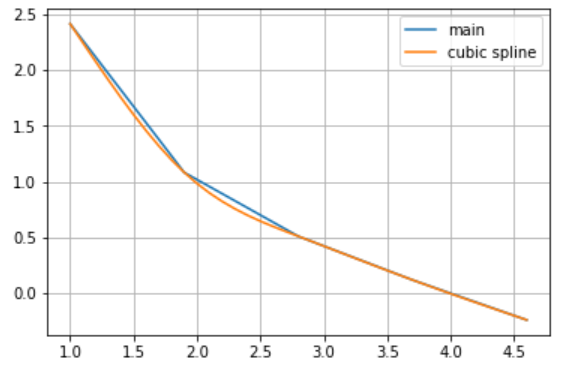
\includegraphics[scale=0.5]{data2.png}

\subsection{Метод наименьших квадратов}

\begin{lstlisting}
def make_spline_matrix(x, y, n, err=10**-5, text=False):
    A, b, n = [], [], n+1
    for i in range(n):
        r = []
        for j in range(n):
            if i == 0 and j == 0:
                r.append(len(x))
            else:
                r.append(sum(map(lambda a: pow(a,i+j),x)))
        A.append(r)
        b.append(sum(map(lambda a,b: pow(a,i) * b,x,y)))
    a_,a = [None] * len(A),[0] * len(A)
    while True:
        for i in range(len(A)):
            s = 0
            for j in range(len(A)):
                if j < i:
                    s += A[i][j] * a_[j]
                elif i != j:
                    s += A[i][j] * a[j]
            a_[i] = (b[i] - s) / A[i][i]
        if sqrt(sum(map(lambda a,b: pow(a - b,2),a,a_))) < err:
            break
        a = copy.copy(a_)
    resx,resy = [],[]
    start = x[0]
    while start < x[-1]:
        resx.append(start)
        resy.append(sum([a_[j] * pow(start, j) for j in range(len(a_))]))
        start += 0.1
    yy = [sum([a_[j] * pow(num, j) for j in range(len(a_))]) for num in x]
    return resx, resy
\end{lstlisting}

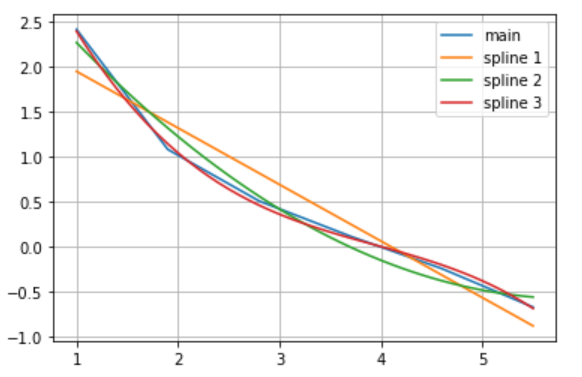
\includegraphics[scale=0.5]{data3.png}

\section{Численное дифференцирование}

\begin{lstlisting}
def find_start(x, p):
    for i in range(0, len(p) - 1):
        if p[i] <= x and x <= p[i + 1]:
            return i

def df1(x, y, x0):
    i = find_start(x0, x)
    elem1 =  (y[i + 1] - y[i]) / (x[i + 1] - x[i])
    elem2 =  ((y[i + 2] - y[i + 1]) / (x[i + 2] - x[i + 1]) - elem1) / (x[i + 2] - x[i]) * (2 * x0 - x[i] - x[i + 1])
    return elem1 + elem2

def df2(x, y, x0):
    i = find_start(x0, x)
    elem1 = (y[i + 2] - y[i + 1]) / (x[i + 2] - x[i + 1])
    elem2 = (y[i + 1] - y[i]) / (x[i + 1] - x[i])
    return 2 * (elem1 - elem2) / (x[i + 2] - x[i])
\end{lstlisting}

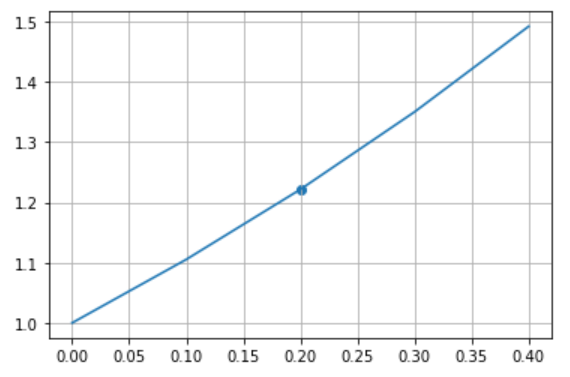
\includegraphics[scale=0.5]{data4.png}

\section{Интегрирование}

\subsection{Проверка методом Рунге-Ромберга}

\begin{lstlisting}
def runge_romberg_richardson(h1, F1, h2, F2, p):
    if h1 < h2:
        return F1 + (F1 - F2) / ((h2 / h1)**p - 1)
    else:
        return F2 + (F2 - F1) / ((h1 / h2)**p - 1)
\end{lstlisting}

\subsection{Метод прямоугольников}

\begin{lstlisting}
def rectangle_integration(a, b, h):
    integ, x = 0.0, a
    while x < b:
        integ += f(x + h / 2)
        x += h
    return h*integ
\end{lstlisting}

\subsection{Метод трапеций}

\begin{lstlisting}
def trapeze_integration(a, b, h):
    integ, x = f(a) / 2, a + h
    while x < b:
        integ += f(x)
        x += h
    return h*(integ + f(x) / 2)
\end{lstlisting}

\subsection{Метод Симпсона}

\begin{lstlisting}
def simpson_integration(a, b, h):
    integ, x = 0.0, a + h
    while x < b:
        integ += f(x - h) + 4*f(x) + f(x + h)
        x += h + h
    return h*integ/3
\end{lstlisting}

\subsection{Зависимость ошибки от шага}

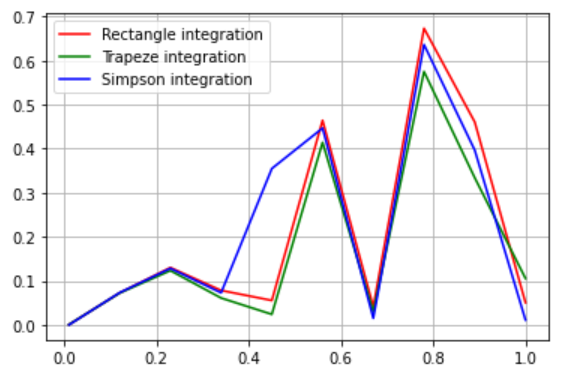
\includegraphics[scale=0.5]{data5.png}

\subsection{Логарифмическая ошибка}

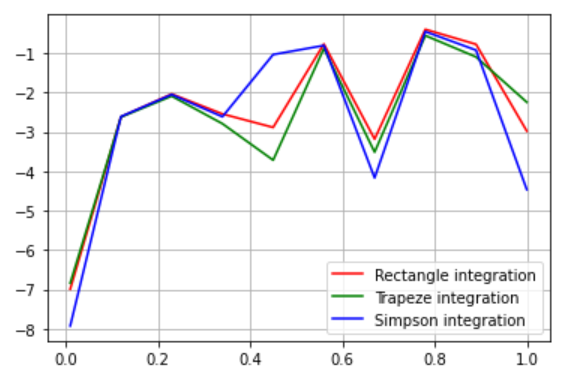
\includegraphics[scale=0.5]{data6.png}

\section{Выводы}

В данной лабораторной работе я научился строить полиномы, сплайны на множестве точек. Научился численному дифференциированию и интегрированию.

\end{document}